\documentclass[11pt]{article}
\usepackage{../common/pbstyle}
\input{../common/sheethead}
\renewcommand{\course}{Ensemble Methods -- TP PAC-Bayes}
\usepackage{needspace}
%% \soltrue is set by the solution wrapper (tp_pacbayes_solutions.tex)
\providecommand{\ifsol}{\iffalse}
\usepackage{comment}
\ifsol
\newtcolorbox{solution}{enhanced,breakable,colback=pbteal!4,colframe=pbteal,boxrule=0.4pt,sharp corners,title={Solution},fonttitle=\bfseries\small,colbacktitle=pbteal!15,coltitle=black}
\else
\excludecomment{solution}
\fi
\newcounter{tppart}
\newcommand{\tppart}[1]{\Needspace{6\baselineskip}\refstepcounter{tppart}\medskip\noindent{\large\bfseries\color{pbblue}Part \thetppart\ -- #1}\par\smallskip}
\newcommand{\code}[1]{\texttt{#1}}
\makeatletter\newcommand\tabinput[1]{\@@input #1 }\makeatother

\begin{document}
\sloppy
\sheethead{TP -- Risk certificates for ensemble methods\ifsol\ -- Solutions\fi}{In this practical session you will
compute PAC-Bayesian risk certificates for random forests, Gibbs posteriors and boosted ensembles on the datasets
of the course, learn the weights of majority votes by minimizing these certificates, and use them for model
selection. The session relies on notebooks~1 to~4 and on the module \code{pbtools.py}. Each part refers to the
corresponding section of the lecture notes. At the end of the session you should have a short report comparing
test risks and certificates, in the same format as in the first practical session.\ifsol{} All the numbers of
these solutions are produced by the script \code{tp\_solutions.py} (also available as a notebook), with
$\delta=0.05$, 5 random stratified $70/30$ splits and forests of $100$ trees trained on bootstrap samples of size
$m/2$; your numbers will differ slightly with other seeds.\fi}

%% =====================================================================
\tppart{Setting up}

\begin{itemize}
\item Download the datasets (\code{datasets.zip}) and the loading script \code{prepdata.py} of the first practical
      session, and the module \code{pbtools.py}. The function \code{data\_recovery(name)} returns a pair
      \code{(X, y)} with labels in $\{0,1\}$: convert them to $\{-1,+1\}$ and standardize the features.
\item Read \code{pbtools.py}: every function is short. It provides the binary kl and its inversions
      (\code{kl\_bin}, \code{kl\_inv\_upper}, \code{kl\_inv\_lower}), the classical bounds (\code{bound\_seeger},
      \code{bound\_mcallester}, \code{bound\_catoni}, \code{bound\_lambda}), a random forest keeping track of its
      out-of-bag samples (\code{BaggedTrees} with \code{oob\_losses}, \code{oob\_tandem}, \code{oob\_disagreement}),
      the majority-vote certificates (\code{fo\_bound}, \code{tnd\_bound}, \code{cbound\_pb}) and two optimizers
      (\code{optimize\_fo}, \code{optimize\_tnd}).
\item Use \textbf{at least 10 datasets}, balanced and imbalanced, for instance \code{australian}, \code{balance},
      \code{bupa}, \code{german}, \code{heart}, \code{iono}, \code{pima}, \code{sonar}, \code{wdbc}, \code{spambase}
      (balanced group) and \code{abalone8}, \code{pageblocks}, \code{satimage}, \code{segmentation}, \code{yeast3}
      (imbalanced group).
\end{itemize}

\begin{solution}
Loading helper used throughout the solutions:
\begin{verbatim}
def load(name):
    X, y = data_recovery(name)
    X = StandardScaler().fit_transform(np.asarray(X, dtype=float))
    return X, np.where(np.asarray(y) > 0, 1, -1)
\end{verbatim}
The sizes range from $208$ (\code{sonar}) to $6435$ (\code{satimage}) examples, and the proportion of positive
examples from $2\%$ to $48\%$. Keep these sizes in mind: a PAC-Bayesian certificate is computed with the number
of examples on which the voters are evaluated, and with only a few hundred examples it cannot be tight.
\end{solution}

%% =====================================================================
\tppart{Warm-up: inverting the kl and certifying one classifier (Section 2)}

\begin{enumerate}
\item Implement the upper inversion $\klup(\hat q,\varepsilon)$ by bisection (Algorithm~1 of the notes) and check it
      against \code{kl\_inv\_upper}.
\item For $m\in\{100,1000\}$, $\delta=0.05$, $\varepsilon=\ln(1/\delta)/m$ and $\hat q\in\{0,0.01,0.05,0.1,0.3,0.5\}$,
      compare three upper confidence bounds on the risk of a \emph{fixed} classifier: Hoeffding $\hat q+\sqrt{\varepsilon/2}$,
      the kl inversion, and the refined Pinsker relaxation $\hat q+\sqrt{2\hat q\varepsilon}+2\varepsilon$. When does the kl
      make a difference?
\item On \code{australian}, split the data in two halves. Learn a decision tree of depth $3$ on the first half and
      compute the Hoeffding and kl test-set bounds of its risk on the second half.
\item Now learn trees of depths $1,\dots,10$ on the first half, keep the one with the smallest error on the second
      half, and compute its kl bound as if it had been fixed in advance. Why is this ``certificate'' not valid? Correct it.
\end{enumerate}

\begin{solution}
\textbf{1.} The bisection keeps an interval $[a,b]$ with $\kl(\hat q\|a)\leq\varepsilon<\kl(\hat q\|b)$, starting from
$[\hat q,1]$; since $p\mapsto\kl(\hat q\|p)$ is increasing on $[\hat q,1]$, halving the interval $30$ times gives
a precision of $10^{-9}$:
\begin{verbatim}
def kl_inv_bisection(q, eps, tol=1e-9):
    a, b = q, 1.0
    while b - a > tol:
        c = (a + b) / 2
        if kl_bin(q, c) > eps: b = c
        else:                  a = c
    return b
\end{verbatim}
It agrees with \code{kl\_inv\_upper} to $10^{-6}$ on all the values of question 2.

\textbf{2.} Results ($\delta=0.05$):
\begin{center}\small
\begin{tabular}{rcccc}
\toprule
$m$ & $\hat q$ & Hoeffding & kl & refined Pinsker \\
\midrule
\tabinput{results/p1_widths.tex}
\bottomrule
\end{tabular}
\end{center}
The Hoeffding width $\sqrt{\ln(1/\delta)/(2m)}$ does not depend on $\hat q$ ($0.122$ for $m=100$, $0.039$ for $m=1000$).
The kl interval is much narrower when $\hat q$ is small: for $\hat q=0$ it is $1-e^{-\varepsilon}\approx\varepsilon$, i.e.\ a
width in $1/m$ instead of $1/\sqrt m$ ($0.003$ instead of $0.039$ for $m=1000$). When $\hat q$ approaches $1/2$ the
two bounds coincide, as predicted by Pinsker's inequality, which is tight around $1/2$. The refined Pinsker bound
is always between the kl and a looser bound, and captures the fast rate. Conclusion: the kl matters for good
classifiers, which is precisely the case of interest.

\textbf{3.} With $n=345$ test examples, the depth-3 tree has a test error of $0.142$, the Hoeffding bound gives
$0.208$ and the kl bound $0.192$ (first numbers of the table of question 4).

\textbf{4.}
\begin{center}\small
\begin{tabular}{cccc|cccc}
\toprule
$n$ & error (depth 3) & Hoeffding & kl & selected depth & its error & naive kl & kl with $\delta/10$ \\
\midrule
\tabinput{results/p1_tree.tex}\\
\bottomrule
\end{tabular}
\end{center}
The selected depth has been chosen because its error on the second half is the smallest: that half is no longer
independent of the selected classifier, and the test-set bound, which holds for a classifier \emph{fixed in
advance}, does not apply (selection bias, Figure~10 of the notes). The correction is the Occam bound with a uniform
prior on the $10$ candidates, i.e.\ a union bound: replace $\delta$ by $\delta/10$, which increases the certificate
from $0.189$ to $0.207$. The price, $\ln 10\approx2.3$ nats, is small; the error would be to pay nothing.
\end{solution}

%% =====================================================================
\tppart{Certificates of a standard random forest (Sections 5 and 7.2)}

For each dataset, repeat 5 times: split the data into $70\%$ training / $30\%$ test (stratified) and learn a
\code{BaggedTrees} forest of 100 trees on the training set with bootstrap samples of size $m/2$.
\begin{enumerate}
\item Compute the test risk of the uniform majority vote, the test Gibbs risk and disagreement, and the three OOB
      certificates (first-order, tandem, C-bound) of the uniform posterior, with $\delta=0.05$. Report also the
      sizes $n_1$ (smallest OOB set) and $n_2$ (smallest intersection of two OOB sets).
\item Check that the certificates are always above the test risk. Which bound is the tightest, on which datasets?
      Relate your answer to the disagreement of the trees (Proposition 5.7) and to $n_1$, $n_2$.
\item Compare the test risk of \code{BaggedTrees} with \code{sklearn.ensemble.RandomForestClassifier}
      (full bootstrap). How much accuracy do we lose by using bootstrap samples of size $m/2$?
\end{enumerate}

\begin{solution}
Mean values over the 5 splits (RF: \code{RandomForestClassifier}; MV, Gibbs, $d$: uniform forest on the test set;
FO, TND, C: OOB certificates of the uniform vote):
\begin{center}\small
\setlength{\tabcolsep}{4pt}
\begin{tabular}{lccccrrccc}
\toprule
dataset & RF & MV & Gibbs & $d$ & $n_1$ & $n_2$ & FO & TND & C-bound \\
\midrule
\tabinput{results/p2_forest.tex}
\bottomrule
\end{tabular}
\end{center}

\textbf{1--2.} All certificates are above the test risk, as they must be (a violation would happen with probability
at most $5\%$ per split). Their quality depends above all on the number of OOB examples. On the small datasets
(\code{bupa}, \code{sonar}, \code{heart}: $n_2<75$) all certificates are vacuous or nearly so: with $54$ examples,
$\ln(2\sqrt{n}/\delta)/n\approx0.09$ even with $\KL=0$, and the factor $2$ or $4$ does the rest. On the larger
datasets (\code{spambase}, \code{pageblocks}, \code{satimage}, \code{segmentation}) they become informative, e.g.\
$0.124$ for \code{pageblocks} whose vote errs on $2.1\%$ of the test points.

Which bound is the tightest? Proposition 5.7 says that, as \emph{oracle} quantities, the C-bound and the tandem bound
beat the first-order bound when $d\geq R(G)$. This condition holds on almost all datasets (compare the columns
Gibbs and $d$), but the certificates tell a different story: the first-order certificate is the smallest on every
dataset except \code{spambase} (on \code{bupa} and \code{sonar} all three are vacuous). The reason is statistical: the tandem bound is estimated on $n_2\approx0.55\,n_1$
examples and multiplied by $4$, and the C-bound needs two kl inversions. Only when the sample is large and the
trees diverse enough (\code{spambase}: $d=0.156>R=0.124$, $n_2=1119$) does the tandem certificate win. The lesson:
the best oracle bound is not necessarily the best certificate.

\textbf{3.} The two forests have very close test risks (e.g.\ $0.051$ vs $0.056$ on \code{spambase}, $0.137$ vs
$0.141$ on \code{australian}); on some datasets \code{BaggedTrees} is even slightly better. Halving the bootstrap
samples costs little accuracy, while it raises the OOB proportions from $e^{-1}\approx37\%$ to $e^{-1/2}\approx61\%$
(and from $14\%$ to $37\%$ for pairs), which makes the certificates much tighter.
\end{solution}

%% =====================================================================
\tppart{Learning the weights (Sections 6 and 7.2)}

\begin{enumerate}
\item On each dataset, compute the posteriors minimizing the first-order bound (\code{optimize\_fo}) and the tandem
      bound (\code{optimize\_tnd}). Report the test risk of the corresponding votes, their certificates and the
      \emph{effective number of trees} $1/\sum_t\rho_t^2$.
\item Produce a table with one row per dataset and, for each posterior (uniform, FO, TND), the mean and standard
      deviation over the 5 splits of the test risk and of the certificate. For the uniform posterior, report the
      best of the three certificates: what correction does this choice require?
\item Which posterior gives the best vote? the best certificate? Are the conclusions of notebook~4 confirmed?
\end{enumerate}

\begin{solution}
Means (standard deviations) over the 5 splits; ``eff.'' is the effective number of trees. For the uniform vote,
the certificate is the minimum of the FO, TND and C-bound certificates computed with $\delta/3$ each (union bound,
Proposition 6.3), since the best bound is chosen after seeing them.
\begin{center}\scriptsize
\setlength{\tabcolsep}{3pt}
\begin{tabular}{l|cc|ccc|ccc}
\toprule
& \multicolumn{2}{c|}{uniform} & \multicolumn{3}{c|}{FO-optimized} & \multicolumn{3}{c}{TND-optimized} \\
dataset & test risk & best cert. & test risk & FO cert. & eff. & test risk & TND cert. & eff. \\
\midrule
\tabinput{results/p3_weights.tex}
\bottomrule
\end{tabular}
\end{center}

\textbf{Best vote.} The TND-optimized vote is as good as the uniform one (mean $0.125$ vs $0.123$, differences
within one standard deviation on every dataset). The FO-optimized vote is worse on all 15 datasets (only marginally on \code{iono}; mean
$0.161$), sometimes by a lot (\code{bupa}: $0.254\to0.367$, \code{sonar}: $0.216\to0.305$). The effective
number of trees explains why: the FO posterior keeps between $2$ and $10$ trees, the TND posterior about $50$ to
$75$. Minimizing a first-order bound selects the individually best trees, which are correlated, and destroys the
diversity that makes the vote work.

\textbf{Best certificate.} Paradoxically, the smallest certificate is almost always the FO certificate of the
FO-optimized posterior (mean $0.486$), because it is estimated on more examples and it minimizes precisely this
number. But it certifies a worse vote. The TND certificate of the TND-optimized posterior is smaller than (or equal to, when both are vacuous) the TND certificate of the uniform vote on every dataset (e.g.\ $0.289\to0.272$ on \code{spambase}), and it becomes the
best compromise when the data are large enough. This reproduces the conclusions of notebook~4 and of Section 7.2:
a certificate that ignores the correlations between voters should not be used as a learning objective for a vote.
\end{solution}

%% =====================================================================
\tppart{The Gibbs posterior and its temperature (Section 4)}

We now build the voters ourselves, so that the prior can be fixed before seeing the data used in the bound.
\begin{enumerate}
\item On \code{wdbc} and \code{australian}, keep $20\%$ of the data to build the voters: all the decision stumps
      $x\mapsto s\,\sign(x_j-\theta)$, $s\in\{\pm1\}$, whose thresholds $\theta$ are the quantiles $10,25,50,75,90\%$ of
      feature $j$ on this part. Split the remaining data into a sample $S$ ($60\%$) used by the bound and a test sample.
\item With the uniform prior, compute the Gibbs posterior $Q_\lambda\propto e^{-\lambda m\widehat R_S(h)}$ for a grid of
      $60$ values of $\lambda$ between $10^{-3}$ and $10^{1.5}$, and plot its empirical Gibbs risk, $\KL(Q_\lambda\|P)/m$ and
      Seeger's bound as functions of $\lambda$.
\item Report the best certificate, the corresponding test Gibbs risk and test risk of the vote, and compare with
      the Occam bound of the stump with the smallest empirical risk. Why is choosing $\lambda$ on the grid free?
\end{enumerate}

\begin{solution}
\begin{center}
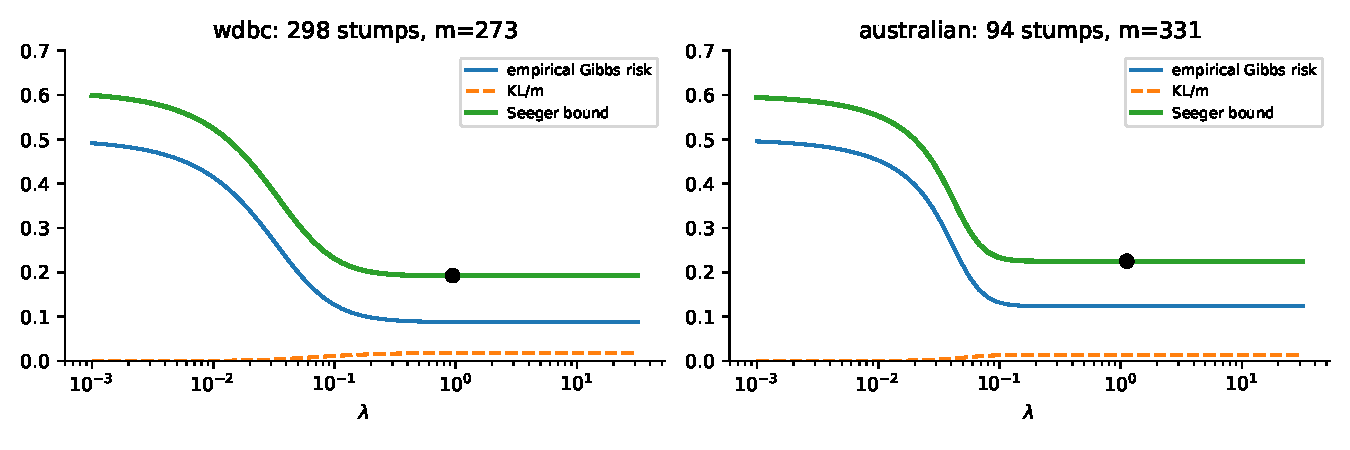
\includegraphics[width=0.9\linewidth]{figures/tp_temperature.pdf}
\end{center}
\begin{center}\small
\setlength{\tabcolsep}{3.5pt}
\begin{tabular}{lrrcccccccc}
\toprule
& & & \multicolumn{5}{c}{best Gibbs posterior} & & \multicolumn{2}{c}{ERM stump (Occam)} \\
dataset & $n$ & $m$ & $\lambda$ & $\widehat R_S(G)$ & KL & Seeger & test Gibbs & test vote & certificate & test \\
\midrule
\tabinput{results/p4_stumps.tex}
\bottomrule
\end{tabular}
\end{center}

\textbf{Shape of the curves.} For small $\lambda$ the posterior is the prior; since every stump comes with its
opposite, the empirical Gibbs risk is exactly $0.5$ and the bound is vacuous. When $\lambda$ grows the empirical
risk drops quickly while $\KL/m$ grows slowly, up to $\ln(n)/m$, and the bound reaches a minimum. Beyond this point
the KL keeps increasing while the empirical risk no longer decreases.

\textbf{Numbers.} The best certificates are $0.192$ (\code{wdbc}) and $0.225$ (\code{australian}), for test Gibbs risks
of $0.104$ and $0.158$. They are obtained for $\lambda\approx1$, where the posterior is already concentrated on a few
stumps ($\KL=4.98$ and $4.54$ nats, close to $\ln n=5.70$ and $4.54$): on these problems a single feature is very
informative, and the best Gibbs posterior is nearly the ERM stump, so its certificate is essentially the Occam
bound ($0.196$ and $0.225$) and its vote is essentially that stump. On these two problems the Gibbs posterior does as well as Occam; it does better when several voters are about equally good, as with the $300$ stumps of \texttt{breast cancer} in Section 4 of the notes.

\textbf{Why is the grid free?} $\lambda$ only indexes posteriors: Seeger's bound holds simultaneously for all $Q$,
hence for all $Q_\lambda$, whatever the way $\lambda$ is chosen (Theorem 6.2). No union bound is needed, contrary
to the parameter $C$ of Catoni's bound (Section 6.3).
\end{solution}

%% =====================================================================
\tppart{Strength versus diversity (Section 5)}

\begin{enumerate}
\item On \code{spambase} and \code{german}, learn forests with \code{max\_features} $\in\{1,\sqrt d,d/2,d\}$
      (3 splits). Report the test Gibbs risk, the test disagreement, the test risk of the vote and the OOB tandem
      and C-bound certificates.
\item Describe how strength and diversity evolve. Which value gives the best vote? Do the certificates follow the
      risk of the vote?
\end{enumerate}

\begin{solution}
\begin{center}\small
\begin{tabular}{llccccc}
\toprule
dataset & \code{max\_features} & Gibbs & $d$ & vote & TND cert. & C-bound cert. \\
\midrule
\tabinput{results/p5_diversity.tex}
\bottomrule
\end{tabular}
\end{center}
Trying more features per split makes each tree stronger (the Gibbs risk decreases, from $0.142$ to $0.114$ on
\code{spambase}) but the trees more similar (the disagreement decreases from $0.192$ to $0.128$). The vote is best
with a single feature on \code{spambase} ($0.048$) and with $d/2$ features on \code{german} ($0.234$): the optimum
is a trade-off, as predicted by the C-bound (Figure~19 of the notes). On \code{spambase} the tandem certificate is
minimal at $\sqrt d$ ($0.291$) and the C-bound certificate decreases and then stabilizes: the certificates see the
trade-off but not its exact optimum, because their estimation error varies with the configuration. On \code{german}
($700$ training examples) the tandem certificate is vacuous and the C-bound certificate hardly informative: with
few examples, certificates cannot guide such a fine choice.
\end{solution}

%% =====================================================================
\tppart{Self-bounding model selection (Section 6)}

\begin{enumerate}
\item On \code{spambase}, \code{pima}, \code{wdbc} and \code{german}, learn $K=5$ forests with \code{max\_depth}
      $\in\{1,2,4,8,\text{None}\}$, minimize the tandem bound of each of them and compute its certificate with $\delta/K$.
      Select the depth with the smallest certificate.
\item Compare with the depth selected by 5-fold cross-validation of the uniform forest on the training set, and
      with the best depth in hindsight (smallest test risk). Report the test risks of the selected models.
\item Why must the certificates be computed with $\delta/K$? When does this selection rule fail, and what should be
      done then?
\end{enumerate}

\begin{solution}
Selected depths on 3 splits, mean test risk of the selected forest, and mean certificate of the model selected by
the certificate:
\begin{center}\small
\setlength{\tabcolsep}{4pt}
\begin{tabular}{lcccccc}
\toprule
dataset & depth (cert.) & test risk & depth (CV) & test risk & best & certificate \\
\midrule
\tabinput{results/p6_selection.tex}
\bottomrule
\end{tabular}
\end{center}
\textbf{Why $\delta/K$.} Keeping the smallest of $K$ certificates is a choice made with the data; the certificate of
the selected model is valid only if all $K$ certificates hold simultaneously, which the union bound guarantees
(Proposition 6.3). The price is $\ln 5\approx1.6$ nats, negligible here.

\textbf{When it works.} On \code{spambase} and \code{wdbc}, where the certificates are informative ($0.29$ and $0.49$),
the certificate selects deep trees and reaches the same test risk as cross-validation, without any validation fold
and with a guarantee on the selected model.

\textbf{When it fails.} On \code{pima} and \code{german}, all the certificates equal $1$: they are vacuous and carry no
information, and the argmin returns the first candidate (depth $1$), which is a poor choice ($0.254$ vs $0.238$ for
cross-validation on \code{pima}, $0.294$ vs $0.247$ on \code{german}). A selection rule based on certificates is
meaningful only when the certificates are non-vacuous: with small samples, one should fall back on
cross-validation (and certify the selected model on a held-out sample), or use a first-order or data-dependent-prior
certificate, which is less loose on small data.
\end{solution}

%% =====================================================================
\tppart{Imbalanced datasets and the balanced error (Section 6)}

The bounds of this course control the 0-1 risk. On imbalanced datasets a trivial classifier predicting the
majority class has a small 0-1 risk.
\begin{enumerate}
\item On the imbalanced datasets, compare the certificates of the uniform forest with the risk of the trivial
      classifier. Are the certificates informative?
\item Obtain a certificate on the \emph{balanced} error
      $\frac12\big(\P(h(x)\neq y\,|\,y=+1)+\P(h(x)\neq y\,|\,y=-1)\big)$: apply the OOB bounds separately to the
      training examples of each class (with $n_+$ and $n_-$ OOB examples) and use a union bound. Implement it and
      comment.
\end{enumerate}

\begin{solution}
\textbf{Construction.} Conditionally on $y=+1$, the examples of the positive class are i.i.d.\ from $\D_{|y=+1}$, and the
OOB construction applies to them: restricting the OOB masks to the positive training examples gives OOB losses
and tandem losses whose expectations are the class-conditional error rates. We compute the FO and TND
certificates on each class with $\delta/4$ (2 classes $\times$ 2 bounds), keep the smallest on each class, and average
them: with probability $\geq1-\delta$ both class-conditional certificates hold, hence their average bounds the
balanced error. In code, it suffices to restrict \code{bt.oob\_} to the columns of the class:
\begin{verbatim}
mask = ytr == cls
saved = bt.oob_; bt.oob_ = saved[:, mask]
L, n1 = bt.oob_losses(Xtr[mask], ytr[mask])
Lt, n2 = bt.oob_tandem(Xtr[mask], ytr[mask])
bt.oob_ = saved
\end{verbatim}
\begin{center}\small
\setlength{\tabcolsep}{4pt}
\begin{tabular}{lccc|cc|cc}
\toprule
& trivial & vote & 0-1 cert. & positives: error & cert. & balanced error & balanced cert. \\
\midrule
\tabinput{results/p7_imbalanced.tex}
\bottomrule
\end{tabular}
\end{center}
\textbf{1.} The trivial classifier has a 0-1 risk equal to the proportion of positives ($0.10$ to $0.14$). The 0-1
certificates of the forest are larger than this value on every dataset, even on \code{pageblocks} ($0.125$ vs $0.102$) where the forest is five times better than the trivial classifier on the test set. In other words, the 0-1 certificates
cannot even guarantee that the forest is better than predicting the majority class.

\textbf{2.} The balanced error reveals what the 0-1 risk hides: on \code{abalone8} the vote misses $93\%$ of the positive
examples and its balanced error ($0.47$) is that of a random guess, although its 0-1 risk is $0.141$. The balanced
certificates are loose, because the positive class contains only a few hundred examples ($0.68$ on \code{pageblocks},
vacuous on three datasets), but they are honest: they certify what matters for an imbalanced problem, and they
show that informative guarantees on the minority class require many minority examples. A natural improvement is to
rebalance the bootstrap samples so that the trees see more positives.
\end{solution}

%% =====================================================================
\tppart{Boosting (Section 7.3)}

AdaBoost also outputs a weighted majority vote. To obtain a certificate, the voters must be evaluated on examples
independent of them.
\begin{enumerate}
\item Split the training set into two halves $S_1,S_2$. Run \code{AdaBoostClassifier} with decision stumps (100
      rounds) on $S_1$, and consider the learned stumps as the voters, with the uniform prior.
\item Compute on $S_2$ the FO and TND certificates of the posterior $\rho_t\propto\alpha_t$ given by AdaBoost (with
      $\delta/2$ each), and of the posteriors minimizing the two bounds. Compare the test risks with those of AdaBoost
      trained on the whole training set.
\item Why are the certificates of the AdaBoost posterior loose, although AdaBoost is accurate? \emph{Hint:} compute the
      Gibbs risk of the stumps on $S_2$ and the KL of the AdaBoost posterior.
\end{enumerate}

\begin{solution}
\begin{center}\scriptsize
\setlength{\tabcolsep}{3pt}
\begin{tabular}{l|cc|cccc|cc|cc}
\toprule
& AdaBoost & AdaBoost & \multicolumn{4}{c|}{AdaBoost posterior on $S_2$} & \multicolumn{2}{c|}{FO-optimized} & \multicolumn{2}{c}{TND-optimized} \\
dataset & (all data) & ($S_1$) & Gibbs & KL & FO cert. & TND cert. & test & FO cert. & test & TND cert. \\
\midrule
\tabinput{results/p8_boosting.tex}
\bottomrule
\end{tabular}
\end{center}
\textbf{2.} Training on half of the data costs AdaBoost almost nothing ($0.148\to0.150$ on \code{australian}). The certificates of
its posterior, however, are vacuous on three datasets and loose on the other two ($0.71$ on \code{wdbc}).
Reweighting the stumps by minimizing the bounds improves the certificates markedly (TND certificate $0.54$ on
\code{australian}, $0.33$ on \code{wdbc}), but mostly at the expense of the vote: the TND-optimized vote errs on
$20\%$ of \code{spambase} instead of $6.5\%$, and on $10\%$ of \code{wdbc} instead of $4.3\%$. The optimized
posteriors concentrate on the few stumps that are good on their own, and lose the combination built by AdaBoost.

\textbf{3.} The explanation lies in the nature of boosting. Its voters are \emph{weak} on purpose: the Gibbs risk of
the stumps on $S_2$ is $0.40$--$0.45$ on four datasets out of five ($0.27$ on \code{wdbc}). AdaBoost makes them accurate \emph{together}, by
putting them in a precise combination with large margins, not by making each of them good. The first-order bound
is then $2\times0.43>0.8$, and the tandem bound, which only uses the joint errors of pairs, cannot see a
combination that relies on many voters at once. The KL of the AdaBoost posterior is small ($0.03$ to $0.4$ nats),
so the complexity is not the problem: the looseness comes from the Gibbs-to-vote relation. This is why boosted votes
are better analysed with margin bounds (Section 5.9), or certified with a hold-out sample: on $S_2$ the test-set
bound of the AdaBoost vote itself would be close to its test risk.
\end{solution}

%% =====================================================================
\tppart{Report}

Summarize your results in a short report (2--3 pages) containing the tables of Parts 3 and 4, one figure of your
choice and a discussion. As in the first practical session, compare methods that are comparable and give standard
deviations; remember that a certificate is not an estimate of the risk, and comment on its tightness, not only on
its value; finally, report every choice made using the data (grids, splits, selected bounds), since each of them may
require a union bound.

\begin{solution}
A good report states the three lessons of the session. First, certificates are only informative when the voters
are evaluated on enough examples (a few thousand OOB examples for a random forest): on small datasets they are
vacuous, and this is not a failure of the implementation. Second, the choice of the bound matters twice: as a
certificate, the first-order bound is often the tightest on small and medium datasets and the tandem bound on large
ones; as a learning objective, only the second-order bound preserves the diversity and the accuracy of the vote.
Third, every data-dependent choice has a price, usually small ($\ln K$), but it must be paid.
\end{solution}

\end{document}
